% !TeX spellcheck = cs_CZ
%{\tikzset{external/prefix={tikz/FYZI/}}
% \tikzset{external/figure name/.add={ch37_}{}}
%=========================== Kapitola: Kvantové chování ===========================================
\setchaptertoc
\chapter{Kvantové chování}\label{fyz:IchapXXXVII}
  \section{Mechanika atomů}\label{fyz:IchapXXXVIIsecI}
    V posledních několika kapitolách jsme se zabývali základními myšlenkami potřebnými k pochopení
    nejdůležitějších světelných jevů, nebo obecně elektromagnetického záření. Zabývali jsme se
    „klasickou teorií“ elektromagnetických vln, která poskytuje adekvátní popis přírody pro velké
    množství jevů. Zatím nás nemuselo znepokojovat, že energie světla se šíří v porcích zvaných
    „fotony“.
    
    Rádi bychom se dál zabývali problémem chování relativně velkých částí hmoty, například jejich
    mechanickými a tepelnými vlastnostmi. Při tomto studiu dojdeme velmi rychle k tomu, že „klasická“
    (nebo starší) teorie velmi rychle selže, neboť hmota se skládá z malých částic s rozměry atomů.
    Přesto se budeme dál zabývat klasickou fyzikou, neboť jen tu můžeme pochopit pomocí klasické
    mechaniky, kterou jsme se učili. Nebudeme však příliš úspěšní. Zjistíme, že na rozdíl od světla se
    v případě látek velmi rychle dostaneme do těžkosti. Atomové jevy bychom mohli nechávat soustavně
    stranou, ale radši si uděláme krátkou exkurzi, v níž si popíšeme základní myšlenky kvantových
    vlastností hmoty, tj. kvantové principy atomové fyziky, abychom získali odhad toho, co budeme
    vynechávat. Některé důležité věci budeme totiž muset vynechat, i když se jim nebudeme moci zcela
    vyhnout.
    
    Podáme tedy jen úvod do kvantové mechaniky, neboť jí samou se budeme zabývat mnohem později.
    
    Kvantová mechanika - to je popis vlastností hmoty ve všech jejích detailech, ale hlavně popis
    toho, co se s ní děje na úrovni atomů. Objekty, které mají velmi malé rozměry, se vůbec nechovají
    tak, jak bychom očekávali na základě naší bezprostřední zkušenosti. Nechovají se jako vlny, ani
    jako částice, nechovají se jako mraky, ani jako kulečníkové koule nebo závaží na pružinách, jako
    nic z toho, co jsme již viděli.

    \begin{figure*}[ht!] %\ref{fyz:fig0922}
      \centering
      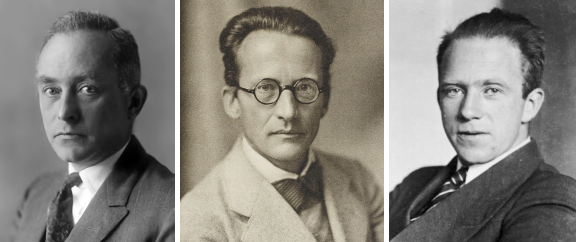
\includegraphics[width=1\linewidth]{fyz_fig0922.png}
      \caption{Zleva: \MaxBorn \ErwinSchrodinger \WernerHeisenberg}
      \label{fyz:fig0922}
    \end{figure*}

    Newton si myslel, že světlo se skládá z částic, ale pak se zjistilo, že se chová jako vlnění.
    Avšak později (začátkem 20. století) se zase ukázalo, že někdy se světlo opravdu chová jako
    částice. Historie objevu elektronu byla taková, že nejdříve se předpokládalo, že se chová jako
    částice a pak se zjistilo, že se chová v mnoha ohledech jako vlna. Takže ve skutečnosti se nechová
    ani tak, ani tak. Dnes už neříkáme, zda se elektron chová jako částice nebo vlna - prostě jsme to
    vzdali. Chová se jako něco úplně jiného.
    
    Existuje však jedno šťastné řešení - elektrony se chovají právě tak jako světlo. Všechny atomové
    objekty (elektrony, protony, neutrony, fotony atd.) se chovají stejně, všechno jsou to „částice -
    vlny“ nebo jak bychom je již nazvali. Proto vše, co se dozvíme o vlastnostech elektronů (které
    budeme používat v našich příkladech), bude platit pro všechny částice včetně fotonů světla.
    
    V první čtvrtině našeho století se nahromadilo o dějích na úrovni atomů a objektů malých rozměrů
    množství informací, které způsobovaly rostoucí zmatek. Jeho vysvětlení podali v letech 1926 a 1927
    Schrödinger, Heisenberg a Born (obr. \ref{fyz:fig0922}). Podařilo se jim získat konzistentní popis
    chování hmoty při velmi malých rozměrech. V této kapitole si probereme základní body tohoto
    popisu.

    Protože se chování atomů vůbec nepodobá tomu, co známe z běžné zkušenosti, je velmi těžké si na ně
    zvyknout a nováčkovi i zkušenému fyzikovi se zdá divné a záhadné. Dokonce ani odborníci ho
    nechápou tak, jak by si přáli. Je to zcela odůvodněné, neboť celá bezprostřední lidská zkušenost a
    intuice platí pro velké objekty. Víme, jak se chovají velké objekty, ale objekty malých rozměrů se
    tak prostě nechovají. Proto se o nich dozvídáme pomocí abstrakce a představivosti, a ne
    prostřednictvím přímé zkušenosti.
    
    V této kapitole se pustíme hned do základních projevů tohoto záhadného chování v jeho
    nejzvláštnější formě. Budeme zkoumat jev, který naprosto nelze vysvětlit žádným klasickým
    způsobem, a který tvoří podstatu kvantové mechaniky. Obsahuje vlastně celou a jedinou záhadu. Tuto
    záhadu nemůžeme vysvětlit. Můžeme si jen říct, jak to funguje a tím si ozřejmíme základní
    zvláštnosti kvantové mechaniky.

  \section{Experiment s kulkami}\label{fyz:IchapXXXVIIsecII}
    Abychom pochopili kvantové chování elektronů, budeme je srovnávat v určitém experimentálním
    uspořádání s chováním takových částic, jako jsou kulky a s chováním vln na vodě. Nejdříve se
    podíváme, jak se v experimentu, zobrazeném na obr. \ref{fyz:fig0426}, budou chovat kulky. Máme
    samopal, který střílí proud kulek. Není příliš přesný, protože rozptyluje kulky náhodně v dosti
    širokém úhlu, jak naznačuje obrázek. Před samopalem je pancéřová deska, jež má dva otvory takové
    velikosti, že jimi může proletět právě jedna kulka. Za ní se nachází ochranná zeď (například z
    tlustého dřeva), která zachytí kulky, jež do ní narazí. Před zdí máme umístěn „detektor“ kulek.
    Může to být krabice naplněná pískem. Každá kulka, která trefí detektor, v něm uvázne. Budeme-li
    chtít, můžeme detektor vyprázdnit a zjistit kolik kulek se v něm zachytilo. Detektor se může
    pohybovat nahoru a dolů (ve směru, který nazveme \(x\)). S tímto zařízením jsme schopni
    experimentálně najít odpověď na otázku: \uv{Jaká je pravděpodobnost toho, že kulka, která
    proletí otvory v desce, dopadne na záchytnou zeď ve vzdálenosti \(x\) od středu ?} Všimněme si
    nejprve, že mluvíme o pravděpodobnosti, neboť neumíme přesně říci, kam určitá kulka dopadne.
    Kulka, jíž se podaří trefit některý z otvorů, se může odrazit od okraje a dopadnout kamkoliv. Pod
    „pravděpodobností“ myslíme možnost, že kulka dopadne na detektor. Můžeme ji určit tak, že
    spočítáme kulky, jež se zachytily v detektoru za určitou dobu a tento počet dělíme celkovým
    počtem kulek, jež za tuto dobu narazily na záchytnou stěnu. Můžeme také předpokládat, že po dobu
    měření střílí samopal stále rovnoměrným tempem, takže hledaná pravděpodobnost bude úměrná počtu
    střel, které dopadly na detektor za nějaký pevně stanovený čas.
    
    \begin{figure}[ht!] %\ref{fyz:fig0426}
      \centering
      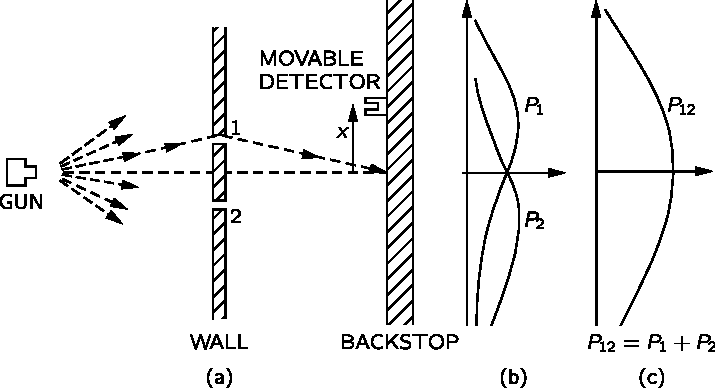
\includegraphics[width=1\linewidth]{fyz_fig0426.pdf}
      \caption{Interferenční experiment s kulkami (\cite[s.~697]{Feynman01})}
      \label{fyz:fig0426}
    \end{figure}

    Pro naše účely bude lepší, když si představíme trochu zidealizovaný experiment, v němž kulky
    nejsou skutečnými kulkami, ale jsou nezničitelné - nemohou se například rozlomit na polovinu. V
    našem experimentu kulky přilétají nepoškozené, a když v detektoru něco najdeme, je to vždy celá
    kulka. Bude-li frekvence výstřelů samopalu malá, zjistíme, že v libovolném okamžiku nedopadne na
    stěnu buď nic nebo jen jedna kulka. Velikost celku tedy nezávisí na kadenci samopalu. Kulky
    přilétají vždy ve stejných celcích. Detektorem měříme pravděpodobnost toho, že přiletí celek.
    Tuto pravděpodobnost měříme jako funkci vzdálenosti \(x\). Výsledek takového měření s tímto
    zařízením (i když jsme měření neprováděli, výsledek si můžeme představit) je zobrazen na grafu
    c) na obr. \ref{fyz:fig0426}. Na grafu nanášíme vodorovně pravděpodobnost a svisle \(x\), takže
    stupnice \(x\) souhlasí s náčrtem zařízení. Tuto pravděpodobnost nazýváme \(P_{12}\) , neboť
    kulky mohly přiletět jedním nebo druhým otvorem. Není nic divného na tom, že \(P_{12}\) je
    největší ve středu grafu a že pro velká \(x\) je velmi malé. Možná se budeme divit, že
    \(P_{12}\) má maximum pro hodnotu \(x= 0\). To lze pochopit, když experiment zopakujeme tak, že
    nejdřív zakryjeme otvor 2 a pak otvor 1. Je-li otvor 2 zakrytý, kulky mohou létat jen prvním
    otvorem a dostaneme křivku, označenou na části b) obrázku jako \(P_1\). Podle očekávaní maximum
    \(P_1\) najdeme pro tu hodnotu \(x\), která leží na přímce spojující samopal a otvor č. 1. Když
    se zakryje otvor č. 1, dostaneme symetrickou křivku zobrazenou jako \(P_2\). Srovnáním částí b)
    a c) na obr. \ref{fyz:fig0426} dostáváme důležitý výsledek
    \begin{equation}\label{fyz:eq591}
      P_{12} = P_1 + P_2
    \end{equation}
    Pravděpodobnosti se prostě sčítají. Výsledek s oběma otevřenými otvory je roven součtu výsledků,
    je-li otevřen jen jeden otvor. Říkáme, že při tom „nenastává interference“, jak uvidíme později.
    Tolik o kulkách, přilétají v celcích a pravděpodobnost jejich dopadu neprojevuje interferenci.
  
  \section{Experiment s vlnami}\label{fyz:IchapXXXVIIsecIII}
    Nyní chceme provést podobný experiment s vlnami. Na obr. \ref{fyz:fig0427} je náčrt
    experimentálního zařízení. Máme koryto s mělkou vodou. Zdrojem vln je nějaký malý předmět poháněný
    motorem nahoru a dolů, který vytváří kruhové vlny. Napravo od zdroje máme opět stěnu \(S\) dvěma
    otvory a za ní je druhá stěna, která je pro jednoduchost „absorbérem“, takže vlny, které na ní
    dopadají, se neodrážejí. Toho lze dosáhnout pomocí postupné pískové „pláže“. Před pláž umístíme
    detektor, který se může pohybovat podél osy \(x\) jako dříve. Jako detektor si můžeme představit
    přístroj k měření výšky vln, jen jeho stupnice bude kalibrována v druhé mocnině skutečné výšky,
    takže jeho údaje budou úměrné energii vlnění nebo také výkonu přenášenému vlněním k detektoru.

    \begin{figure}[hb!] %\ref{fyz:fig0427}
      \centering
      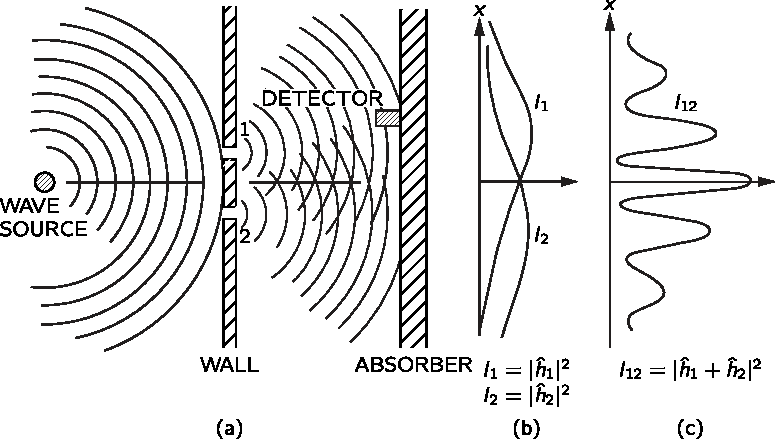
\includegraphics[width=1\linewidth]{fyz_fig0427.pdf}
      \caption{Interferenční experiment s vlnami na vodě (\cite[s.~697]{Feynman01})}
      \label{fyz:fig0427}
    \end{figure}

    První věc, jíž je třeba si všimnout, je to, že intenzita vlnění může nabýt libovolnou velikost.
    Pokud se zdroj hýbe jen velmi málo, je vlnění u detektoru velmi slabé. Když se zdroj pohybuje
    víc, je i intenzita vlnění u detektoru větší. Intenzita vlny může nabývat jakoukoliv hodnotu.
    Nemohli bychom říci, že energie se přenáší v jakýchsi „celcích“.
    
    Nyní změřme intenzitu vln pro různé hodnoty \(x\) za předpokladu, že zdroj vlnění pracuje stále
    rovnoměrně. Dostaneme zajímavý výsledek označený na obrázku (část c) jako křivka \(I_{12}\).
    Vznik takového průběhu jsme odvodili při studiu interference elektromagnetických vln. V tomto
    případě bychom viděli, že na otvorech nastává difrakce původní vlny a od každého otvoru se šíří
    nové kruhové vlny. Zakryjeme-li na chvíli jeden z otvorů a změříme rozložení intenzity podél
    absorbéru, dostaneme dost jednoduché křivky, znázorněné na obrázku v části b). \(I_1\) je
    intenzita vlny z otvoru 1 (kterou měříme tak, že otvor 2 je zakryt) a \(I_2\) je intenzita vlny
    z otvoru 2 (při zavřeném otvoru 1).

    Intenzita \(I_{12}\), kterou pozorujeme, když jsou oba otvory otevřeny, určitě není rovna součtu
    \(I_1\) a \(I_2\). Říkáme, že dochází k „interferenci“ dvou vln. Na některých místech (kde má
    křivka \(I_{12}\) maxima) jsou vlnění „ve fázi“, součet amplitud je velký a je tedy velká i
    intenzita. Taková „konstruktivní interference“ nastane všude tam, kde je vzdálenost detektoru od
    jednoho otvoru větší (nebo menší) o celý násobek vlnové délky než vzdálenost detektoru od
    druhého otvoru.

    Na místech, kam dopadnou vlny s fázovým rozdílem 1: (kde jsou v proti fázi), bude výsledné
    vlnění v detektoru rovno rozdílu obou amplitud. Vlny „interferují destruktivně“ a pro intenzitu
    vlny dostáváme malou hodnotu. Tak malé hodnoty dostaneme všude tam, kde se vzdálenost otvoru 1
    od detektoru liší od vzdálenosti k otvoru 2 o lichý násobek poloviny vlnové délky. Malé hodnoty
    \(I_{12}\) na obr. \ref{fyz:fig0427} odpovídají místům, kde vlny interferují destruktivně. 

    Určitě si pamatujeme, že vztah mezi \(I_{1}\), \(I_{2}\) a \(I_{12}\)  lze vyjádřit takto:
    Okamžitou výšku vody v detektoru od vlny z otvoru 1 lze zapsat jako \(\hat{h}_1e^{\imath\omega
    t}\) (z toho reálná část), kde amplituda \(\hat{h}_1\) je obecně komplexní číslo. Intenzita je
    úměrná střední hodnotě druhé mocniny výšky nebo pomocí komplexních čísel \(\abs{\hat{h}_1}^2\).
    Podobně pro otvor 2 je výška rovna \(\hat{h}_2e^{\imath\omega t}\)  a intenzita je úměrná
    \(\abs{\hat{h}_2}^2\). Jsou-li otevřeny oba otvory, výšky vln se sčítají \((\hat{h}_1 +
    \hat{h}_2)e^{\imath\omega t}\)  a intenzita je \(\abs{\hat{h}_1 + \hat{h}_2}^2\). Pro naše účely
    můžeme vynechat konstantu úměrnosti, takže pro interferující vlny máme vztahy:
    \begin{equation}\label{fyz:eq592}
      I_1 = \abs{\hat{h}_1}^2, \quad I_2 = \abs{\hat{h}_2}^2, \quad 
      I_{12} = \abs{\hat{h}_1 + \hat{h}_2}^2.
    \end{equation}
    Vidíme, že výsledek se zcela liší od toho, co jsme dostali pro kulky (rovnice \ref{fyz:eq591}).
    Umocníme-li \(\abs{\hat{h}_1 + \hat{h}_2}^2\), vidíme, že
    \begin{equation*}
      I_{12} = \abs{\hat{h}_1 + \hat{h}_2}^2 
             = \abs{\hat{h}_1}^2 + \abs{\hat{h}_2}^2 + 2\abs{\hat{h}_1}\abs{\hat{h}_2}\cos\delta.
    \end{equation*}
    kde \(\delta\) je fázový rozdíl mezi \(\hat{h}_1\) a \(\hat{h}_2\). Pomocí intenzit můžeme
    napsat
    \begin{equation}\label{fyz:eq593}
      I_{12} = I_1 + I_2 + 2\sqrt{I_1I_2}\cos\delta.
    \end{equation}
    Poslední člen v (\ref{fyz:eq593}) je „interferenční člen“. Tolik, pokud jde o vlny na vodě.
    Intenzita může nabývat jakoukoliv hodnotu a projevuje interferenci.

  \section{Experiment s elektrony}\label{fyz:IchapXXXVIIsecIV}
    Nyní si představíme podobný experiment s elektrony. Je znázorněn na obr. \ref{fyz:fig0428}.
    Použijeme elektronové dělo, jež se skládá z elektricky žhaveného wolframového vlákna obklopeného
    kovovou krabicí s otvorem. Má-li drát záporné napětí vzhledem ke krabici, budou elektrony
    emitované drátem urychlovat směrem ke krabici a některé z nich proletí otvorem. Všechny elektrony
    vyletující z děla budou mít (přibližně) stejnou energii. Před dělem je opět stěna (z tenkého
    plechu) s dvěma otvory. Za ní se nachází další deska, která slouží k zachytávání elektronů. Před
    ní umístíme pohyblivý detektor. Detektorem může být Geigerův počítač nebo ještě lépe, elektronový
    násobič napojený na reproduktor.

    \begin{figure}[ht!] %\ref{fyz:fig0428}
      \centering
      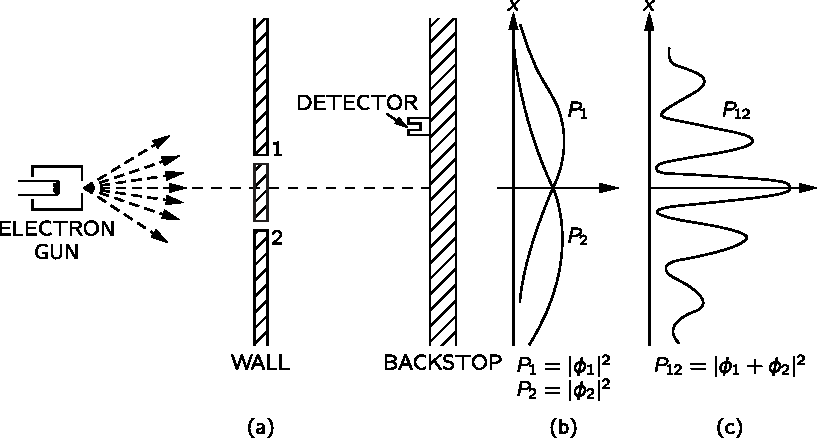
\includegraphics[width=1\linewidth]{fyz_fig0428.pdf}
      \caption{Interferenčni experiments elektrony
              (\cite[s.~697]{Feynman01})}
      \label{fyz:fig0428}
    \end{figure}

    Hned na začátku musíme říci, abyste se nepokoušeli tento experiment sestavit (na rozdíl od
    předcházejících dvou). Tento experiment se nikdy takto nedělal. Obtíž spočívá v tom, že k tomu,
    aby se projevily pro nás zajímavé efekty, muselo by mít zařízení neskutečně malé rozměry.
    Provádíme „myšlený experiment“, který jsme si vybrali proto, že se o něm dá snadno přemýšlet.
    Výsledky známe, neboť bylo provedeno mnoho experimentů v takových měřítkách a rozměrech, že se v
    nich popisované jevy projevily.
    
    První věc, které si v našem experimentu s elektrony všimneme, je ta, že z detektoru (tj. z
    reproduktoru) slyšíme ostrá „cvaknutí“. Všechna „cvaknutí“ jsou stejná. Neexistují „polocvaknutí
    “. Také si všimneme, že „cvaknutí“ jsou velmi nepravidelná; něco jako: cvak ... cvak - cvak ...
    cvak ... cvak ... cvak - cvak ... cvak ... atd., jistě jste to slyšeli, když pracoval Geigerův
    počítač. Počet cvaknutí, jež napočítáme za dostatečně dlouhou dobu, dejme tomu za mnoho minut,
    bude vždy přibližně stejný. Můžeme mluvit o průměrném tempu, s jakým je slyšet cvaknutí (v
    průměru tolik a tolik cvaknutí za minutu).

    Při posunování detektoru se tempo cvakání buď zrychluje nebo zpomaluje, ale velikost (hlasitost)
    každého cvaknutí je stejná. Snížíme-li teplotu vlákna v děle, tempo cvakání se zpomalí, ale
    stále zní každé cvaknutí stejně. Všimli bychom si také, že když použijeme dva nezávislé
    detektory, cvakne jeden nebo druhý, ale nikdy ne oba najednou. (Leda že by občas následovala dvě
    cvaknutí tak rychle za sebou, že by je naše ucho nemuselo rozlišit.) Cokoliv tedy dopadá na
    zachycovač, dopadá v „celcích“. Všechny „celky“ mají stejnou velikost: přilétají jen úplné
    „celky“ a přilétají na zachycovač jednotlivě. Říkáme: „Elektrony vždy přilétají ve stejných
    celcích.“ 
    
    Podobně jako u našeho experimentu s kulkami můžeme jít dál a experimentálně najít odpověď na
    otázku, jaká je relativní pravděpodobnost toho, že elektronový „celek“ dopadne na zachycovač v
    různých vzdálenostech \(x\) od středu. Jako již dříve relativní pravděpodobnost dostaneme
    sledováním tempa cvakání při rovnoměrné činnosti děla. Pravděpodobnost, že celky dopadnou do
    určitého bodu \(x\), je úměrná střednímu tempu cvakání v bodě \(x\).
    
    Výsledkem našeho experimentuje zajímavá křivka označená jako \(P_{12}\) na obr.
    \ref{fyz:fig0428}. Ano. Tak se chovají elektrony.

  \section{Interference elektronových vln}\label{fyz:IchapXXXVIIsecV}
    Pokusme se analyzovat křivku na obr. \ref{fyz:fig0428}, abychom viděli, zda můžeme pochopit toto
    chování elektronů. První, co bychom řekli, je, že přilétají-li elektrony v celcích, přilétají
    buď otvorem 1 nebo otvorem 2. Zformujeme to jako předpoklad:
    
    \emph{Předpoklad A}: Každý elektron prochází bud' otvorem 1 nebo otvorem 2.
    
    Na základě předpokladu A všechny elektrony, které doletí na zachycovač, můžeme rozdělit do dvou
    tříd: 1) na ty, které přiletěly otvorem 1 a 2) na ty, co přiletěly otvorem 2. Takže naměřená
    křivka musí být dána součtem efektů od elektronů, které přiletěly otvorem 1 a od elektronů,
    které přiletěly otvorem 2. Ověřme si to experimentem. Nejdříve budeme měřit elektrony, které
    přiletí otvorem 1. 0tvor 2 uzavřeme a spočítáme cvakání v našem detektoru. Z tempa cvakání
    dostaneme \(P_1\). Výsledek měření je znázoměn křivkou označenou na obr. \ref{fyz:fig0428}b) jako
    \(P_1\). Výsledek se zdá být celkem rozumný. Stejným způsobem měříme \(P_2\), rozložení
    pravděpodobnosti pro elektrony, které přiletěly otvorem 2. Výsledek tohoto experimentu je také
    znázorněn na obrázku.
    
    Je jasné, že výsledek \(P_{12}\), získaný, když byly oba otvory otevřeny, není součtem
    pravděpodobností \(P_1\) a \(P_2\) pro každý otvor zvlášť. Analogicky s naším vlnovým
    experimentem můžeme říci: „Existuje tady interference.“ Pro elektrony:
    \begin{equation*}
      P_{12} \neq P_1 + P_2
    \end{equation*}

    Jak může dojít k takové interferenci? Snad bychom měli říci: „Dobře, to znamená, že
    pravděpodobně není pravda, že celky letí jedním nebo druhým otvorem, neboť, kdyby to byla
    pravda, pravděpodobnosti by se měly sčítat. Možná, že letí nějakým komplikovanějším způsobem.
    Rozdělí se na polovinu a ...“ Ale ne! Nemohou se rozdělit, vždy přilétají v celcích ... „Dobře,
    snad některé z nich projdou otvorem 1 a pak projdou kolem otvorem 2 a tak několikrát dokola nebo
    letí po nějaké jiné komplikované dráze... pak, tím že zakryjeme otvor 2, změníme celkové
    možnosti a elektron, který začal letět otvorem 1, nakonec dopadne na zachycovač ...“ Ale
    všimněme si! Existují takové body, do nichž přiletí velmi málo elektronů, když jsou otevřeny oba
    otvory, ale když jeden z nich zavřeme, přiletí do nich mnoho elektronů, takže zakrytím jednoho
    otvoru se zvýší počet od druhého otvoru. Je třeba si také všimnout, že ve středu křivky je
    \(P_{12}\) víc než dvakrát větší než \(P_1+P_2\). Vypadá to tak, jako by se zakrytím jednoho
    otvoru snížil počet elektronů, které přilétávají druhým otvorem. Tyto dva jevy lze těžko
    vysvětlit tím, že by elektrony letěly po složitějších dráhách.
    
    Je to úplně záhadné a čím víc na to myslíme, tím se to zdá záhadnější. Bylo vymyšleno mnoho
    teorií k vysvětlení křivky \(P_{12}\)  pomocí jednotlivých elektronů letících otvory po
    komplikovaných dráhách, ale ani jedna nebyla úspěšná. Žádná neumí získat správnou křivku
    \(P_{12}\)  pomocí \(P_1\)  a \(P_2\).
    
    Přesto je matematika dávající do souvislosti \(P_1\)  a \(P_2\) s \(P_{12}\)  mimořádně
    jednoduchá, což je dost překvapující. \(P_{12}\)  se podobá \(I_{12}\) z obr. \ref{fyz:fig0427}a
    tam to bylo jednoduché. Co se děje na zachycovači lze popsat pomocí dvou komplexních čísel,
    která můžeme nazvat \(\hat{\varphi}_1\) a \(\hat{\varphi}_2\) (samozřejmě, že jsou funkcemi
    \(x\)). Druhá mocnina absolutní hodnoty \(\hat{\varphi}_1\)  dává výsledek, pro otvor 1, tj.
    \(P_1=\abs{\hat{\varphi}_1}^2\). Výsledek, pro otvor 2, je dán podobně jako
    \(P_2=\abs{\hat{\varphi}_2}^2\), a výsledek pro oba otvory je \(P_{12}=\abs{\hat{\varphi}_1 +
    \hat{\varphi}_12}^2\). Je to stejná matematika, kterou jsme měli pro vlny na vodě! (Tak
    jednoduchý výsledek by se dal těžko získat tím, že elektrony by létaly otvory sem a tam po
    nějakých komplikovaných dráhách.)
    
    Můžeme tedy udělat závěr: Elektrony přilétají v celcích jako částice a pravděpodobnost dopadu
    těchto celků je rozložena jako rozložení intenzity vlny. V tomto smyslu se elektron chová „někdy
    jako částice a někdy jako vlna“.
    
    Mimochodem, když jsme se zabývali klasickými vlnami, definovali jsme intenzitu jako časovou
    střední hodnotu druhé mocniny amplitudy a komplexní čísla jsme použili jako trik ke zjednodušení
    analýzy. Ale z kvantové mechaniky vychází, že amplitudy musí být reprezentovány komplexními
    čísly. Jen reálná část nepostačuje. Zatím je to jen technický rozdíl, neboť jinak vypadají
    vzorce úplně stejně.
    
    Je-li pravděpodobnost příletu oběma otvory dána tak jednoduše, i když ne jako součet \(P_1\)  a
    \(P_2\), není k tomu vlastně už co dodat. S tím, že se příroda chová takovým způsobem, souvisí
    mnoho drobných záludností. Rádi bychom si nyní některé z nich ilustrovali. Za prvé, protože
    počet elektronů, které dopadnou do určitého bodu není roven počtu těch, které proletí otvorem 1,
    plus těch, které proletí otvorem 2, jak plyne z předpokladu A. Předpoklad A tedy neplatí. Není
    pravda, že elektron musí letět buď otvorem 1 nebo otvorem 2. Toto tvrzení lze ověřit dalším
    experimentem.
      
  \section{Sledování elektronů}\label{fyz:IchapXXXVIIsecVI}
    Pokusíme se provést následující experiment: Do naší elektronové aparatury přidáme velmi silný
    zdroj světla a umístíme ho za stěnu s otvory, těsně mezi ně, jak je ukázáno na obr.
    \ref{fyz:fig0429}. Víme, že elektrické náboje rozptylují světlo, takže, když elektron proletí na
    své cestě k detektoru kolem zdroje, část světla se na něm rozptýlí i do našeho oka, a tak
    uvidíme, kudy elektron letí. Když například elektron poletí po dráze otvorem 2, měli bychom
    vidět světelný záblesk vycházející z blízkosti bodu A na obr. \ref{fyz:fig0429}. Když elektron
    poletí přes otvor 1, budeme očekávat, že uvidíme záblesk v blízkosti horního otvoru. Kdyby se
    stalo, že světlo uvidíme na obou místech současně, protože elektron se rozdělil na poloviny …
    Proveďme už ten experiment!
    \begin{figure}[ht!] %\ref{fyz:fig0429}
      \centering
      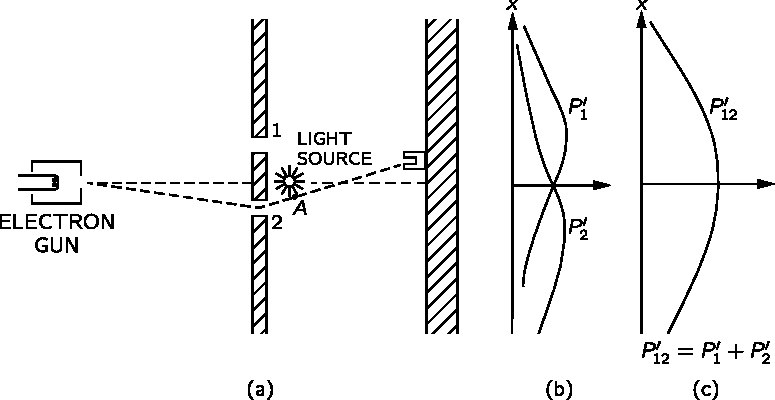
\includegraphics[width=1\linewidth]{fyz_fig0429.pdf}
      \caption{Jiný experiment s elektrony (\cite[s.~697]{Feynman01})}
      \label{fyz:fig0429}
    \end{figure}

    Vidíme toto: vždy, když slyšíme „cvaknutí“ z našeho elektronového detektoru (na zachycovači),
    vidíme také světelný záblesk buď v blízkosti otvoru 1 nebo blízko otvoru 2, ale nikdy ne u obou
    současně! Výsledek je vždy stejný, bez ohledu na to, kde máme detektor. Z tohoto pozorování
    můžeme vyvodit závěr, že sledujeme-li elektrony, vidíme, že procházejí jedním nebo druhým
    otvorem. Experimentálně je tedy potvrzeno, že předpoklad A musí platit.
    
    Kde je potom chyba v našem argumentu proti tvrzení A? Proč prostě \(P_{12}\) není rovno
    \(P_1+P_2\)? Vraťme se k experimentu. Sledujme dráhy elektronů a zjistíme, co se s nimi děje. V
    každé poloze \(x\) detektoru spočítáme dopadající elektrony a také si pomocí sledování záblesků
    všimneme, kterým otvorem přiletěly. Můžeme si o tom vést takové záznamy: Vždy, když budeme
    slyšet „cvaknutí“ a uvidíme záblesk v blízkosti otvoru 1, uděláme čárku v prvním sloupci a když
    uvidíme záblesk v blízkosti otvoru 2, uděláme čárku v druhém sloupci. Každý elektron je
    zaznamenán v některé ze dvou tříd: mezi těmi, které proletěly otvorem 1 nebo mezi těmi, které
    proletěly otvorem 2. Z čísel zaznamenaných ve sloupci 1, dostaneme pravděpodobnost \(P_1'\), že
    elektron přiletí na detektor otvorem 1 a z čísel zaznamenaných ve sloupci 2 dostaneme \(P_2'\),
    pravděpodobnost toho, že elektron dopadne na detektor otvorem 2. Zopakujeme-li toto měření pro
    mnoho hodnot \(x\), dostaneme křivky \(P_1'\) a \(P_2'\) znázorněné na obr. \ref{fyz:fig0429}b).
    
    To není ani tak překvapující! Pro \(P_1'\) dostáváme něco velmi podobného tomu, co jsme předtím
    dostali pro \(P_1'\) zakrytím otvoru 2 a \(P_2'\) je podobné tomu, co jsme dostali zakrytím
    otvoru 1. Takže odpadají všechny komplikované záležitosti jako průchod oběma otvory.
    Sledujeme-li elektrony, vidíme, že prolétají otvory tak, jak to od nich očekáváme. Ať už jsou
    otvory zavřené nebo otevřené, ty, které vidíme přiletět otvorem 1, mají stejné rozložení, bez
    ohledu na to, zda je otvor zavřený nebo otevřený.
    
    Ale počkejme! Co nyní dostáváme pro celkovou pravděpodobnost? Pravděpodobnost toho, že elektrony
    dopadnou na detektor libovolnou cestou? Tuto informaci už máme. Prostě se zatváříme, jako bychom
    se nikdy nedívali na světelné záblesky a sečteme impulzy detektoru, jež jsme měli rozděleny do
    dvou sloupců. Musíme sčítat jenom tato čísla. Pro pravděpodobnost, že elektron přiletí na
    zachycovač libovolným otvorem máme \(P_{12}' = P_1' + P_2'\). Takže při sledování toho, kterým
    otvorem naše elektrony prolétají, již nedostáváme známou interferenční křivku \(P_{12}\), ale
    novou \(P_{12}'\), v níž se neprojevuje interference! Když světlo vypneme, dostaneme opět
    \(P_{12}\).

    Musíme udělat závěr, že když se na elektrony díváme, jejich rozložení na zachycovači je jiné,
    než když se na ně nedíváme. Narušila se snad celá věc tím, že jsme zapnuli světelný zdroj? Musí
    to být tak, že elektrony jsou velmi jemné a světlo tím, že se na nich rozptyluje, do nich „strčí
    “ a tím se změní jejich pohyb. Víme, že elektrické pole světla působící na elektron se projeví
    silou pohybující elektronem. Možná jsme měli očekávat takovou změnu pohybu. V každém případě má
    světlo na elektrony velký vliv. Tím, že jsme se pokusili elektrony „sledovat“, změnili jsme
    jejich pohyb. To znamená, že náraz, který elektron pocítí, když se na něm rozptyluje foton, je
    takový, že dokáže dostatečně změnit pohyb elektronu, takže, když měl letět do bodu, kde má
    \(P_{12}\) maximum, přiletěl tam, kde má minimum. To je důvod, proč už nevidíme interferenční
    efekty.
    
    Možná si myslíme: „Nepoužívejme tak silný zdroj! Zmenšeme jeho jas! Světelné vlny potom budou
    slabší a nebudou tak silně elektrony rušit. Určitě, čím bude světlo slabší a slabší, tím budou
    světelné vlny slabší a slabší, až budou mít zanedbatelný efekt.“ Dobře, zkusme to. První věc,
    které si všimneme, je ta, že záblesky světla rozptýleného na elektronech letících kolem se
    nezeslabují. Jsou to vždy stejně velké záblesky. Jediná věc, která se stane při zmenšování jasu
    světla, je ta, že někdy slyšíme „cvaknutí“ v detektoru, ale nevidíme žádný záblesk. Elektron
    proletěl kolem, aniž bychom ho viděli. Pozorujeme jen to, že světlo se projevuje podobně jako
    elektrony; věděli jsme, že je to vlnění, nyní zjišťujeme, že jsou to také „částice“. Vždy
    přiletí nebo se rozptyluje v celcích, které nazýváme „fotony“. Zmenšením intenzity světelného
    zdroje nezměníme velikost fotonů, jen počet emitovaných fotonů za jednotku času. To vysvětluje,
    proč při slabém zdroji některé elektrony proletí kolem, aniž bychom je viděli. Když elektron
    letěl kolem, právě tam nebyl žádný foton.

    Trochu to odstrašuje. Je-li pravda, že vždy, když „vidíme“ elektron, vidíme záblesk stejné
    velikosti, pak vidíme vždy jen ty elektrony, jejichž pohyb byl světlem ovlivněn. Zkusme provést
    takový experiment se slabým světlem. Uslyšíme-li nyní cvaknutí v detektoru, uděláme si o tom
    záznam v některém ze tří sloupců: Ve sloupci 1 pro elektrony, jež vidíme u otvoru 1, ve sloupci
    2 pro elektrony, jež vidíme u otvoru 2 a ve sloupci 3 pro elektrony, jež jsme vůbec neviděli.
    Zpracujeme-li tyto údaje (vypočítáme pravděpodobnosti), dostaneme tyto výsledky: Elektrony,
    které jsme „viděli u otvoru 1“ mají rozdělení jako \(P_1'\); ty, jež jsme „viděli u otvoru 2“,
    mají rozdělení jako \(P_2'\) (takže ty, které jsme „viděli bud' u otvoru 1 nebo u otvoru 2 “
    mají rozdělení jako) a ty, které jsme vůbec neviděli, mají „vlnové“ rozložení jako je \(P_{12}\)
    na obr. \ref{fyz:fig0428}! \emph{Když elektrony nevidíme, máme interferenci!}
    
    Je to pochopitelné. Když elektron nevidíme, žádný foton na něj nepůsobil a když ho vidíme,
    působil na něj foton. Toto působení je vždy stejné, neboť světelné fotony vyvolávají vždy stejně
    velký záblesk a rozptyl fotonů je dostatečně silný jev k tomu, aby zrušil jakýkoliv
    interferenční efekt.
    
    Neexistuje nějaký způsob, jak uvidět elektrony aniž bychom je ovlivnili? V jedné z
    předcházejících kapitol jsme se dozvěděli, že hybnost, kterou má „foton“, je nepřímo úměrná
    vlnové délce (\(p= h/\lambda\)). Náraz, který pocítí elektron od fotonu při jeho rozptylu směrem
    do našeho oka, závisí určitě na velikosti hybnosti fotonu. Když jsme chtěli elektrony ovlivnit
    jen slabě, neměli jsme zmenšovat intenzitu světla, ale frekvenci (to je totéž jako zvětšení
    vlnové délky). Použijme světlo červenější barvy! Můžeme dokonce použít infračervené „světlo“
    nebo rádiové vlny (jako radar) a „zjistit“ kudy letěl elektron pomocí nějakého zařízení, které
    může „vidět světlo“ takových vlnových délek. Použitím jemnějšího „světla“ se snad vyhneme
    silnému ovlivňování elektronů.
    
    Zkusme provést celý experiment s delšími vlnami. Budeme ho několikrát opakovat vždy se „světlem
    “, které má větší vlnovou délku. Zpočátku se zdá, že se nic nemění. Výsledky jsou stále stejné.
    Pak se stane strašná věc. Jistě si pamatujeme, jak jsme si řekli, když jsme mluvili o
    mikroskopu, že vzhledem k vlnové povaze světla existuje určité omezení pro vzdálenost dvou bodů,
    abychom je mohli ještě vidět jako dvě oddělené tečky. Tato vzdálenost je řádově rovna vlnové
    délce světla. Proto, když je nyní vlnová délka větší, než je vzdálenost mezi otvory, vidíme při
    rozptylu světla elektrony rozmazaný záblesk a už nemůžeme říci, kterým otvorem elektron
    proletěl. Víme jen to, že někde proletěl. A právě pomocí „světla“ této barvy zjistíme, že nárazy
    na elektrony jsou tak slabé, že \(P_{12}'\) se začíná podobat \(P_{12}\) - začneme registrovat
    nějakou interferenci. Ovlivnění elektronů světlem bude dostatečně malé, až když jsou vlnové
    délky „světla“ mnohem delší než vzdálenost mezi otvory (kdy už nemáme žádnou možnost určit, kudy
    elektron proletěl), a tehdy opět dostaneme křivku \(P_{12}\) znázorněnou na obr.
    \ref{fyz:fig0428}.

    \begin{figure}[ht!] %\ref{fyz:fig0430}
      \centering
      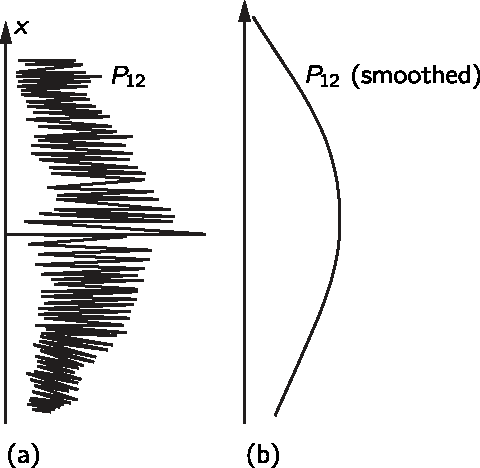
\includegraphics[width=0.8\linewidth]{fyz_fig0430.pdf}
      \caption{Interferenční obrazs kulkami: a) skutečný, b) pozorovaný (\cite[s.~697]{Feynman01})}
      \label{fyz:fig0430}
    \end{figure}

    Zjišťujeme, že v našem experimentu nelze světlo nastavit tak, aby se dalo určit, kudy elektron
    proletěl a aby se současně nezměnilo rozložení pravděpodobnosti. Heisenberg naznačil, že nové
    zákony přírody mohou být konzistentní, jen když existují nějaká základní omezení našich
    experimentálních schopností, která jsme si předtím neuvědomovali. Jako obecný princip navrhl
    Heisenberg svůj \emph{princip neurčitosti}, který v řeči našeho experimentu můžeme zformulovat
    takto: „Nelze zkonstruovat takové zařízení, pomocí něhož bychom mohli určit, kterým otvorem
    proletěl elektron, aniž bychom elektrony neovlivnili natolik, že by se porušil interferenční
    obraz.“ Když nějaké zařízení dokáže určit, kterým otvorem elektron proletěl, nemůže být tak
    dostatečně jemné, že by se podstatně neporušil interferenční obraz. Nikdo nikdy nenašel ani
    nevymyslel způsob, jak by bylo možné princip neurčitosti obejít. Musíme proto předpokládat, že
    popisuje základní vlastnost přírody.
    
    Řeknete: „Dobře, ale co bude s předpokladem A? Je pravda nebo není, že elektron prochází bud'
    otvorem 1 nebo otvorem 2? Jediná odpověď', kterou máme je ta, že pomocí experimentu jsme
    zjistili, že k tomu, abychom se nedostali do rozporu, musíme přemýšlet určitým zvláštním
    způsobem. Abychom se vyhnuli nesprávným předpovědím, musíme mluvit takto:“ Díváme-li se na
    otvory, nebo přesněji, máme-li zařízení, jež může určit, zda elektron prochází otvorem 1 nebo 2,
    lze říci, že prochází bud' otvorem 1 nebo otvorem 2. Ale když se nepokoušíme určit, kudy jdou
    elektrony, když nic nemůže v experimentu elektrony ovlivnit, nelze říci, zda elektrony jdou
    otvorem 1 nebo otvorem 2. Kdyby to někdo řekl a začal z toho vyvozovat závěry, dopustí se ve své
    analýze chyby. To je logické „lano“, po němž musíme balancovat, chceme-li úspěšně popsat
    přírodu.

    Když se pohyb hmoty - včetně elektronů - musí popsat pomocí vln, co potom platí pro naše kulky z
    prvního experimentu? Proč tam nevidíme interferenční obraz? Z vlnového popisu vyplývá, že vlnové
    délky kulek jsou tak nepatrné, že interferenční obraz je velmi jemný. Tak jemný, že oddělená
    maxima a minima nelze rozeznat žádným detektorem s konečnými rozměry. Viděli jsme jen určitý
    průměr, jenž dává klasickou křivku. Na obr. \ref{fyz:fig0430} jsme se pokusili schematicky
    naznačit, jak to vypadá pro velkorozměrné objekty. V části a) je znázorněno rozložení
    pravděpodobnosti, které lze předpovědět pro kulky pomocí kvantové mechaniky. Rychlé kmity by
    měly představovat interferenční obraz od takových velmi krátkých vln. Avšak libovolný fyzikální
    detektor zabírá vždy několik vlnových délek a měření dává hladkou křivku nakreslenou na obrázku
    v části b).

  \twocolumn[\section{Základní principy kvantové mechaniky}\label{fyz:IchapXXXVIIsecVII}]
    Napíšeme shrnutí hlavních závěrů z našich experimentů, ale upravíme si je do takové formy, aby
    platily obecně, pro všechny takové experimenty. Naše shrnutí bude úspěšnější, když si nejprve
    definujeme „ideální experiment“ jako takový, v němž se neprojevují neurčité vnější vlivy, s
    nimiž nemůžeme počítat. Budeme zcela přesní, když řekneme: „Ideální experiment je ten
    experiment, v němž jsou všechny počáteční i konečné podmínky přesně definovány.“ „Události“
    budeme obecně nazývat určitou množinu počátečních a konečných podmínek. (Například: „Elektron
    vyletí z děla, dopadne na detektor a nic jiného se nestane.“) Přistupme tedy ke shrnutí našich
    poznatků:
        
    \begin{mdframed}[style=highlight]
      \begin{center}
        SHRNUTÍ
      \end{center}
      \begin{itemize}[noitemsep]
        \item Pravděpodobnost \(P\) toho, že v ideálním experimentu nastane nějaká událost, je dána
              druhou mocninou absolutní hodnoty komplexního čísla \(\varphi\), jež se nazývá
              amplitudou pravděpodobnosti \(\varphi\)
              \begin{equation}\label{fyz:eq595}
                P = \abs{\varphi}^2
              \end{equation}
        \item Může-li nějaká událost nastat několika způsoby, je amplituda pravděpodobnosti takové
              události rovna součtu amplitud pravděpodobností pro každý způsob uvažovaný zvlášť.
              Nastává interference.  
              \begin{subequations}\label{fyz:eq594}
                \begin{equation}
                  \varphi = \varphi_1+\varphi_2,        \label{fyz:eq594a}
                \end{equation}
                \begin{equation} 
                  P = \abs{\varphi_1+\varphi_2}^2.      \label{fyz:eq594b}
                \end{equation}
              \end{subequations}
        \item Lze-li v daném experimentu určit, která z možností skutečně nastala, je
              pravděpodobnost události rovna součtu pravděpodobností pro každou alternativu.
              Interference se ztrácí.
              \begin{equation}\label{fyz:eq596}
                P = P_1 + P_2
              \end{equation}
      \end{itemize}        
    \end{mdframed}

    Můžeme se stále ptát: \uv{Jak to funguje? Jaký se za tímto zákonem skrývá mechanizmus?} Nikdo za
    tímto zákonem nenašel žádný mechanizmus. Nikdo neumí víc „vysvětlit“ než jsme si právě
    „vysvětlili“. Nikdo neumí dát nějaký hlubší pohled na tuto situaci. Nemáme ani nejmenší potuchu
    o existenci nějakého fundamentálnějšího mechanizmu, z něhož by bylo možné odvodit tyto výsledky.
    
    \emph{Rádi bychom zdůraznili velmi důležitý rozdíl, který je mezi klasickou a kvantovou
    mechanikou.} Mluvili jsme o pravděpodobnosti toho, že za daných okolností přiletí elektron.
    Předpokládali jsme, že v našem experimentu (nebo třeba v tom nejdokonalejším), by bylo nemožné
    exaktně předpovědět, co se stane. Můžeme předpovídat jen pravděpodobnost! To by znamenalo, je-li
    to opravdu tak, že fyzika se vzdala možnosti pokusit se exaktně předpovědět, co se stane za
    daných okolností. Ano, fyzika se toho vzdala! Nevíme, jak předpovědět, co se stane za daných
    okolností, a nyní věříme, že je to nemožné, a že jediné, co lze předpovědět, jsou
    pravděpodobnosti různých událostí. je třeba uznat, že je to ústupek od našeho dřívějšího ideálu
    poznání přírody. Může to být krok zpět, ale nikdo nepřišel na to, jak by se dal obejít.
    
    Uvedeme několik poznámek o jednom návrhu, který někdy slýcháme, jak se pokusit vyhnout uvedenému
    popisu. Lze ho vyjádřit takto: „Elektron má možná nějaký vnitřní pohyb - nějaké vnitřní proměnné
    - o němž zatím ještě nevíme. Snad to bude důvod, proč neumíme předpovědět, co se stane.
    Kdybychom se mohli na elektron podívat víc zblízka, snad bychom uměli povědět, kam dopadne.“
    Podle toho, co dosud víme, je to nemožné. Vznikne nová obtíž. Předpokládejme, že uvnitř
    elektronu pracuje jakýsi mechanizmus, který určuje, kam elektron dopadne. Tento mechanizmus musí
    také rozhodnout, kterým otvorem elektron poletí na své cestě. Nesmíme však zapomenout, že to co
    je uvnitř elektronu, by nemělo záviset na tom, co děláme, například na tom, zda otevřeme nebo
    zakryjeme některý z otvorů. Takže, když se elektron rozhodne ještě před startem: a) který otvor
    použije, b) kam dopadne; pro elektrony, které si zvolily otvor 1, bychom měli dostat \(P_1\),
    pro elektrony, které si zvolily otvor 2, bychom měli dostat \(P_2\) a pro elektrony, které
    proletí oběma otvory, bychom měli nevyhnutně dostat součet \(P_1 + P_2\). Zdá se, že to by
    nebylo možné obejít. Právě jsme si ale experimentálně ověřili, že tak tomu není. Nikdo nenašel
    řešení této hádanky. Proto se musíme v současnosti omezit na výpočet pravděpodobnosti. Říkáme „v
    současnosti“, ale máme velmi silné podezření, že je to něco, co s námi zůstane navždy - že je
    nemožné rozluštit tuto záhadu - že příroda skutečně taková je.

  \section{Princip neurčitosti}\label{fyz:IchapXXXVIIsecVIII}
    Heisenberg původně vyjádřil princip neurčitosti takto: Měříme-li nějaký objekt a přitom dokážeme
    určit jeho složku hybnosti ve směru osy \(x\) s nepřesností \(\Delta p\), nemůžeme současně
    poznat složku jeho polohy \(x\) s větší přesností než \(\Delta x = h/\Delta p\). Součin
    neurčitosti polohy a hybnosti v kterémkoliv okamžiku musí být větší než Planckova konstanta. Je
    to vyjádření zvláštního případu principu neurčitosti, který jsme již uvedli v obecnější formě:
    Nelze zkonstruovat zařízení, jež by určilo, která ze dvou možností vznikla aniž by současně
    nedošlo k porušení interferenčního obrazu.

    \begin{figure}[ht!] %\ref{fyz:fig0431}
      \centering
      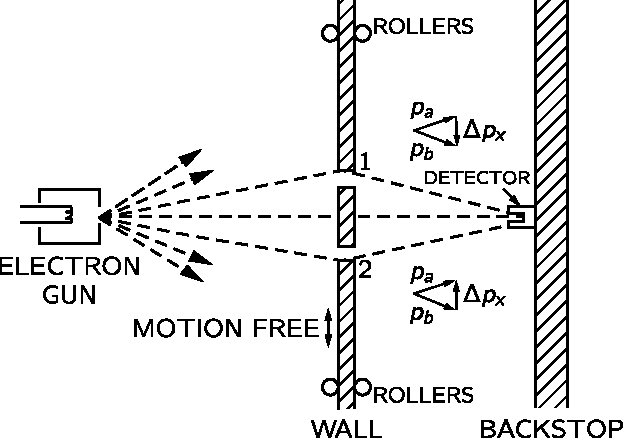
\includegraphics[width=1\linewidth]{fyz_fig0431.pdf}
      \caption{Experiment, v němž se měří zpětnýráz stěny (\cite[s.~697]{Feynman01})}
      \label{fyz:fig0431}
    \end{figure}

    Na jednom zvláštním případě si ukažme, že Heisenbergův princip neurčitosti musí platit,
    nechceme-li se dostat do těžkostí. Představme si, že experiment z obr. \ref{fyz:fig0429} upravíme
    tak, že stěnu s otvory upevníme na válečky, na nichž se může volně pohybovat nahoru a dolů (ve
    směru osy \(x\)), jak je to na obr. \ref{fyz:fig0431}. Pozorným sledováním pohybů stěny se můžeme
    pokusit určit, kterým z otvorů elektron prošel. Představme si, co se stane, je-li detektor
    umístěn v poloze \(x= 0\). Očekávali bychom, že elektron, jenž prochází otvorem 1, musí být
    stěnou odchýlen směrem dolů, aby dopadl na detektor. Když se změní svislá složka hybnosti
    elektronu, musí se stěna odrazit opačným směrem se stejnou hybností. Stěna pocítí náraz směrem
    vzhůru. Prochází-li elektron dolním otvorem, měla by stěna pocítit náraz směrem dolů Je jasné,
    že pro libovolnou polohu detektoru bude odevzdaná hybnost stěně jiná, když elektron poletí
    otvorem 1, než když poletí otvorem 2. Takže sledováním pohybu stěny můžeme snadno říci, kterou
    dráhu elektron použil, aniž bychom elektrony ovlivnili.

    Abychom to mohli udělat, musíme znát hybnost stěny předtím, než jí proletí elektron. Změříme-li
    její rychlost po průletu elektronu, můžeme určit změnu hybnosti stěny. Pamatujme, že podle
    principu neurčitosti nemůžeme současně znát s libovolnou přesností polohu stěny a její hybnost.
    Neznáme-li však přesnou polohu stěny, nevíme ani přesně, kde se nacházejí oba otvory. Pro každý
    elektron budou na jiném místě. To znamená, že pro každý elektron bude střed interferenčního
    obrazu jinde. Rychlé změny interferenčního obrazu se takto smažou. V další kapitole si ukážeme
    kvantitativně, že určíme-li dostatečně přesně hybnost stěny, abychom podle zpětného rázu
    zjistili, který otvor byl použit, potom bude podle principu neurčitosti neurčitost v poloze
    stěny \(x\) dost velká, aby se obraz na detektoru posouval nahoru a dolů ve směru osy \(x\) o
    vzdálenost, jež je rovna přibližně vzdálenosti maxima od vedlejšího minima. Tyto náhodné posuny
    stačí k tomu, aby se obraz rozmazal natolik, že nevidíme žádnou interferenci.
    
    Princip neurčitosti „ochraňuje“ kvantovou mechaniku. Heisenberg si uvědomil, že kdyby se dala
    změřit současně hybnost i poloha s větší přesností, kvantová mechanika se zhroutí. Proto
    vyslovil domněnku, že to musí být nemožné. Mnoho lidí se pokoušelo vymyslet nějaký způsob, jak
    by se to dalo udělat, ale nikdo nedokázal vymyslet, jak změřit polohu i hybnost čehokoliv -
    stěny, elektronu, kulečníkově koule, atd. - s větší přesností. Kvantová mechanika si zachovává
    svou ohroženou, ale odůvodněnou existenci.

  \section{Příklady a cvičení}\label{fyz:IchapXXXVIIsecIX}
   
%~~~~~~~~~~~~~~~~~~~~~~~~~~~~~~~~~~~~~~~~~~~~~~~~~~~~~~~~~~~~~~~~~~~~~~~~~~~~~~~~~~~~~~~~~~~~~~~~~~